% Name: Price ceiling
% Description: A legal maximum price set below equilibrium: buyers want more than sellers will supply, leaving a shortage, and the trades lost form a deadweight loss.
% Tags: price ceiling, shortage, rent control, deadweight loss, microeconomics

\usetikzlibrary{arrows.meta}

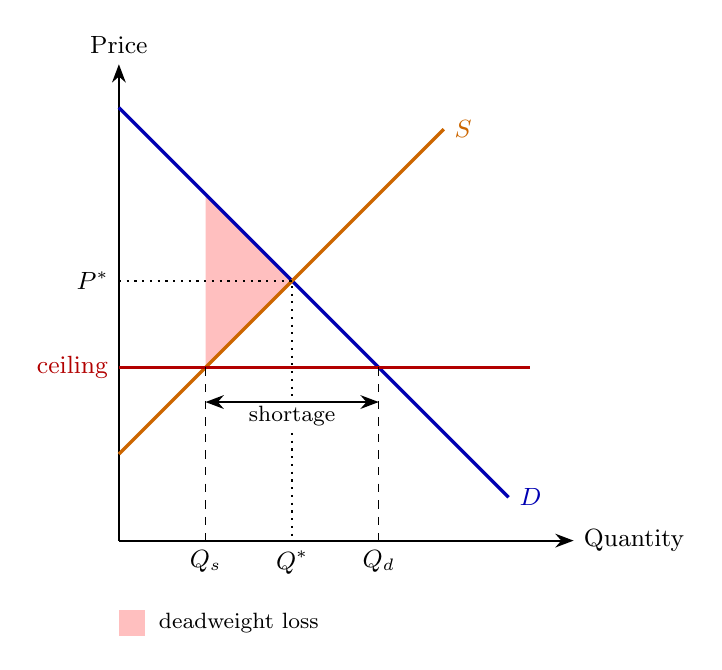
\begin{tikzpicture}[>={Stealth}, scale=0.55, every node/.style={font=\small}]
  % D: P = 10 - Q, S: P = 2 + Q; at the ceiling P = 4, sellers supply 2 and buyers demand 6
  \fill[red!25] (2,8) -- (2,4) -- (4,6) -- cycle;
  \draw[->, thick] (0,0) -- (10.5,0) node[right] {Quantity};
  \draw[->, thick] (0,0) -- (0,11) node[above] {Price};
  \draw[very thick, blue!70!black] (0,10) -- (9,1) node[right] {$D$};
  \draw[very thick, orange!80!black] (0,2) -- (7.5,9.5) node[right] {$S$};
  \draw[very thick, red!70!black] (0,4) node[left] {ceiling} -- (9.5,4);
  \draw[dashed] (2,4) -- (2,0) node[below] {$Q_s$} (6,4) -- (6,0) node[below] {$Q_d$};
  \draw[dotted, thick] (0,6) node[left] {$P^*$} -| (4,0) node[below] {$Q^*$};
  \draw[<->, thick] (2,3.2) -- node[below, fill=white, inner sep=1pt, font=\footnotesize] {shortage} (6,3.2);
  % Swatches under the axis name the shaded areas
  \fill[red!25] (0,-2.2) rectangle ++(0.6,0.6);
  \node[anchor=west, font=\footnotesize] at (0.7,-1.9) {deadweight loss};
\end{tikzpicture}
